
The $W$-boson polarization affects the lepton decay angles, and in turn the transverse momentum of the leptons.
A general expression for the fully differential distribution of the charged lepton is 
\begin{eqnarray}
\frac{d\sigma}{d\pTW dy dm d\Omega}  & = & \frac{d\sigma}{d\pTW dy dm} [(1 + \cos^2\theta) \nonumber \\
 & + &  \frac{1}{2} A_0 (1-3\cos^2\theta) + A_1 \sin 2\theta \cos\phi  \nonumber \\
 & + & \frac{1}{2}A_2 \sin^2\theta\cos 2\phi + A_3 \sin\theta\cos\phi \nonumber \\
 & + & A_4 \cos\theta + A_5 \sin^2\theta\sin 2\phi \nonumber \\
 & + & A_6 \sin 2\theta\sin\phi + A_7 \sin\theta\sin\phi ],
\label{eq:wai}
\end{eqnarray}
where the decay angles $\theta, \phi$ are expressed in the Collins-Soper (C-S) frame~\cite{Collins:1977iv},
and the $A_i$ coefficients depend on the \pT, rapidity, and invariant mass of the $\ell\nu$ system.  The 
coefficients can be calculated perturbatively in $\alpha_{\mathrm{S}}$, with $A_5,~A_6$, and $A_7$ becoming non-zero
only at NNLO in QCD.  The $A_0$ term primarily reflects the relative fractions of the $qq\to W$, $qg\to Wq$, and
higher-order subprocesses, and has a significant \pTW~dependence while being nearly independent of boson rapidity.
The $A_4$ term produces a forward-backward asymmetry, and is thus sensitive to the directions of the incoming
quark and anti-quark in the dominant $q\bar{q}' \to W$ process. It depends on rapidity and on the PDF set used
in the calculation, and decreases with increasing \pTW. 

The \textsc{ResBos-C} and \textsc{ResBos-CP} codes resum a subset of contributions to Equation~\ref{eq:wai},
specifically those affecting the $(1 + \cos^2\theta)$ and $A_4 \cos\theta$ terms.  This partial resummation modifies
the $A_0$--$A_3$ terms relative to fixed-order predictions, as demonstrated in Figure~\ref{fig:aiplots}, where
$A_0-A_3$ are shown for $W$-boson events generated at $\sqrt{s}=1.96$~TeV with \textsc{ResBos-C}, \textsc{ResBos-CP},
\textsc{ResBos2}, and \textsc{DYNNLO}.  The partial-resummation predictions differ with respect to measurements
performed at the LHC~\cite{STDM-2014-10}, which instead agree with fully-resummed calculations such as
\textsc{ResBos2} or {\sc Wj-MiNNLO}, and fixed-order calculations such as \textsc{DYNNLO}.  

Experimental fits for $m_W$ in data use theoretical predictions of the leptonic angular distributions from
\textsc{ResBos-C} for CDF, \textsc{ResBos-CP} for D0, \textsc{DYNNLO}~\cite{Catani:2007vq,Catani:2009sm} for
ATLAS, and DYTurbo for LHCb.  The CDF experiment applies a post-fit correction to reproduce the NNPDF3.1 PDF
prediction, and this correction includes the effect of updating the angular coefficients to those calculated
by \textsc{ResBos2}.  

In order to achieve a common theoretical treatment of the $W$-boson polarization, the results of the CDF and 
D0 fits to the measurement distributions are adjusted to correspond to the \textsc{ResBos2} calculation of the 
leptonic angular distributions at ${\cal O}(\alpha_{\mathrm{S}})$.  Events generated with \textsc{ResBos-C} or
\textsc{ResBos-CP} 
are reweighted such that the $A_0-A_4$ coefficients match those of \textsc{ResBos2}, as functions of \pTW~and 
$y_W$.  The $W$-boson \pT~is fixed to that of the original measurement, in the same manner as for the 
$\delta m_W^{\scriptsize\textrm{PDF}}$ evaluations in Sec.~\ref{sec:corrPDF}.  The impact of the reweighting on
the CDF \mT~and \pTl~distributions is shown in Fig.~\ref{fig:airewCDF}, and the $\delta m_W^{\mathrm{pol}}$
values from reweighting
the $A_i$ coefficients individually and together are given in Tables~\ref{tab:aireweightcdf}~and~\ref{tab:aireweightd0}
for CDF and D0, respectively.  The reweighting procedure reproduces the direct fit from \textsc{ResBos-C} or
\textsc{ResBos-CP} to \textsc{ResBos2}, as expected since the basis of spherical harmonics is complete and exact.
The results of the reweighting procedure for the D0 
configuration, $\delta m_W^{\mathrm{pol}} = -6.4$, $-6.9$, and $-15.8$~MeV for the \mT, \pTl, and
\met~distributions, respectively, are applied to the measured $m_W$.  For CDF, values of
$\delta m_W^{\mathrm{pol}} = -9.5$, $-8.4$, and $-12.5$~MeV for the \mT, \pTl, and
\met~distributions, respectively, are applied to events generated with \textsc{ResBos-C}.
%All uncertainties are statistical.

ATLAS estimates a 5.8 MeV polarization modelling uncertainty based on the precision of measurements on the 
$Z$-boson resonance, while the LHCb uncertainty of 10 MeV arises from its determination of the $A_3$ 
coefficient as part of its fit for $m_W$.  These uncertainties are taken to be uncorrelated.  The Tevatron 
experiments do not include a corresponding uncertainty in their measurements.  An uncorrelated uncertainty 
is applied to the shift calculated for each experiment to account for the limitations of the parameterized MWWG
simulation.  This uncertainty is $\approx 1$~MeV and is similar to that obtained by taking the difference between
the NLO and NNLO fixed-order calculations of the leptonic angular coefficients.

\begin{figure}[!tbp]
  \centering
  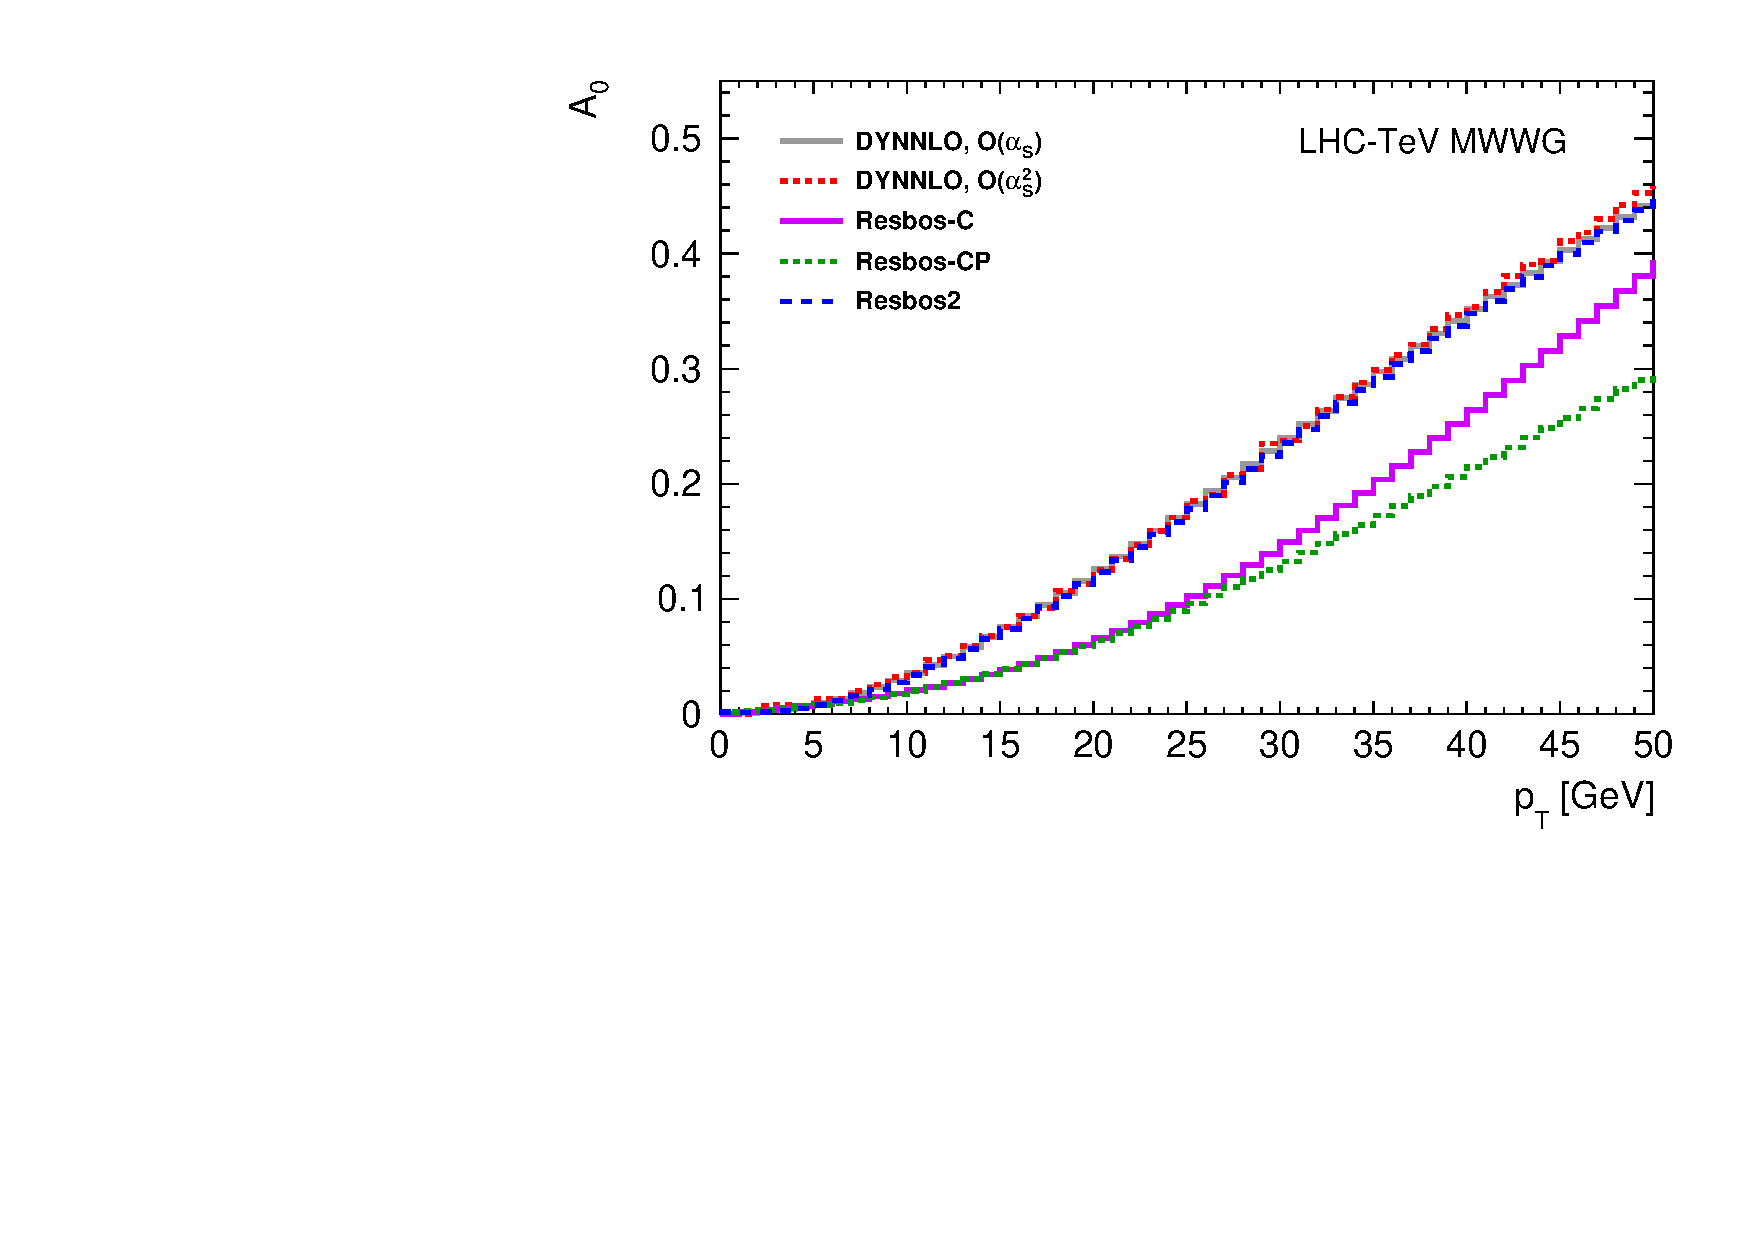
\includegraphics[width=0.88\columnwidth]{a0_pt.pdf}
  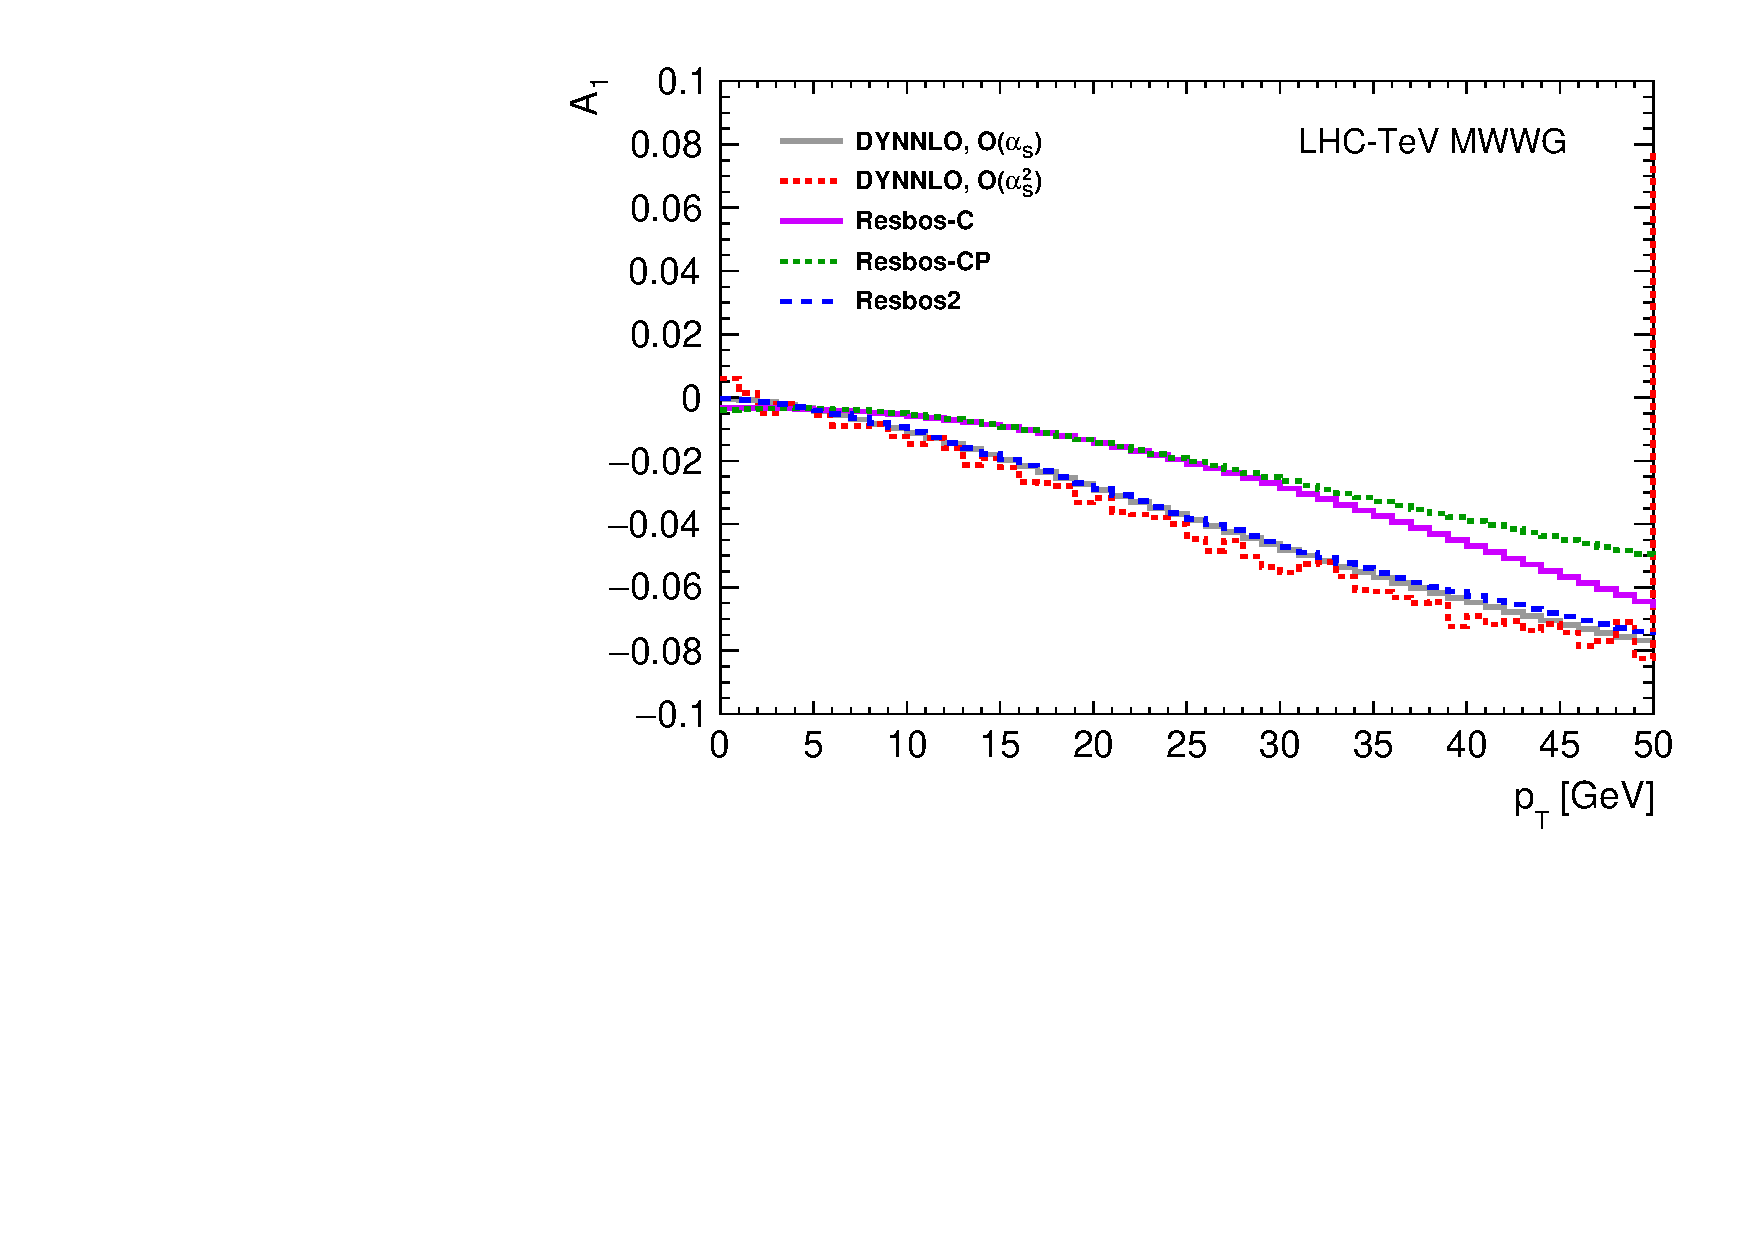
\includegraphics[width=0.88\columnwidth]{a1_pt.pdf}
  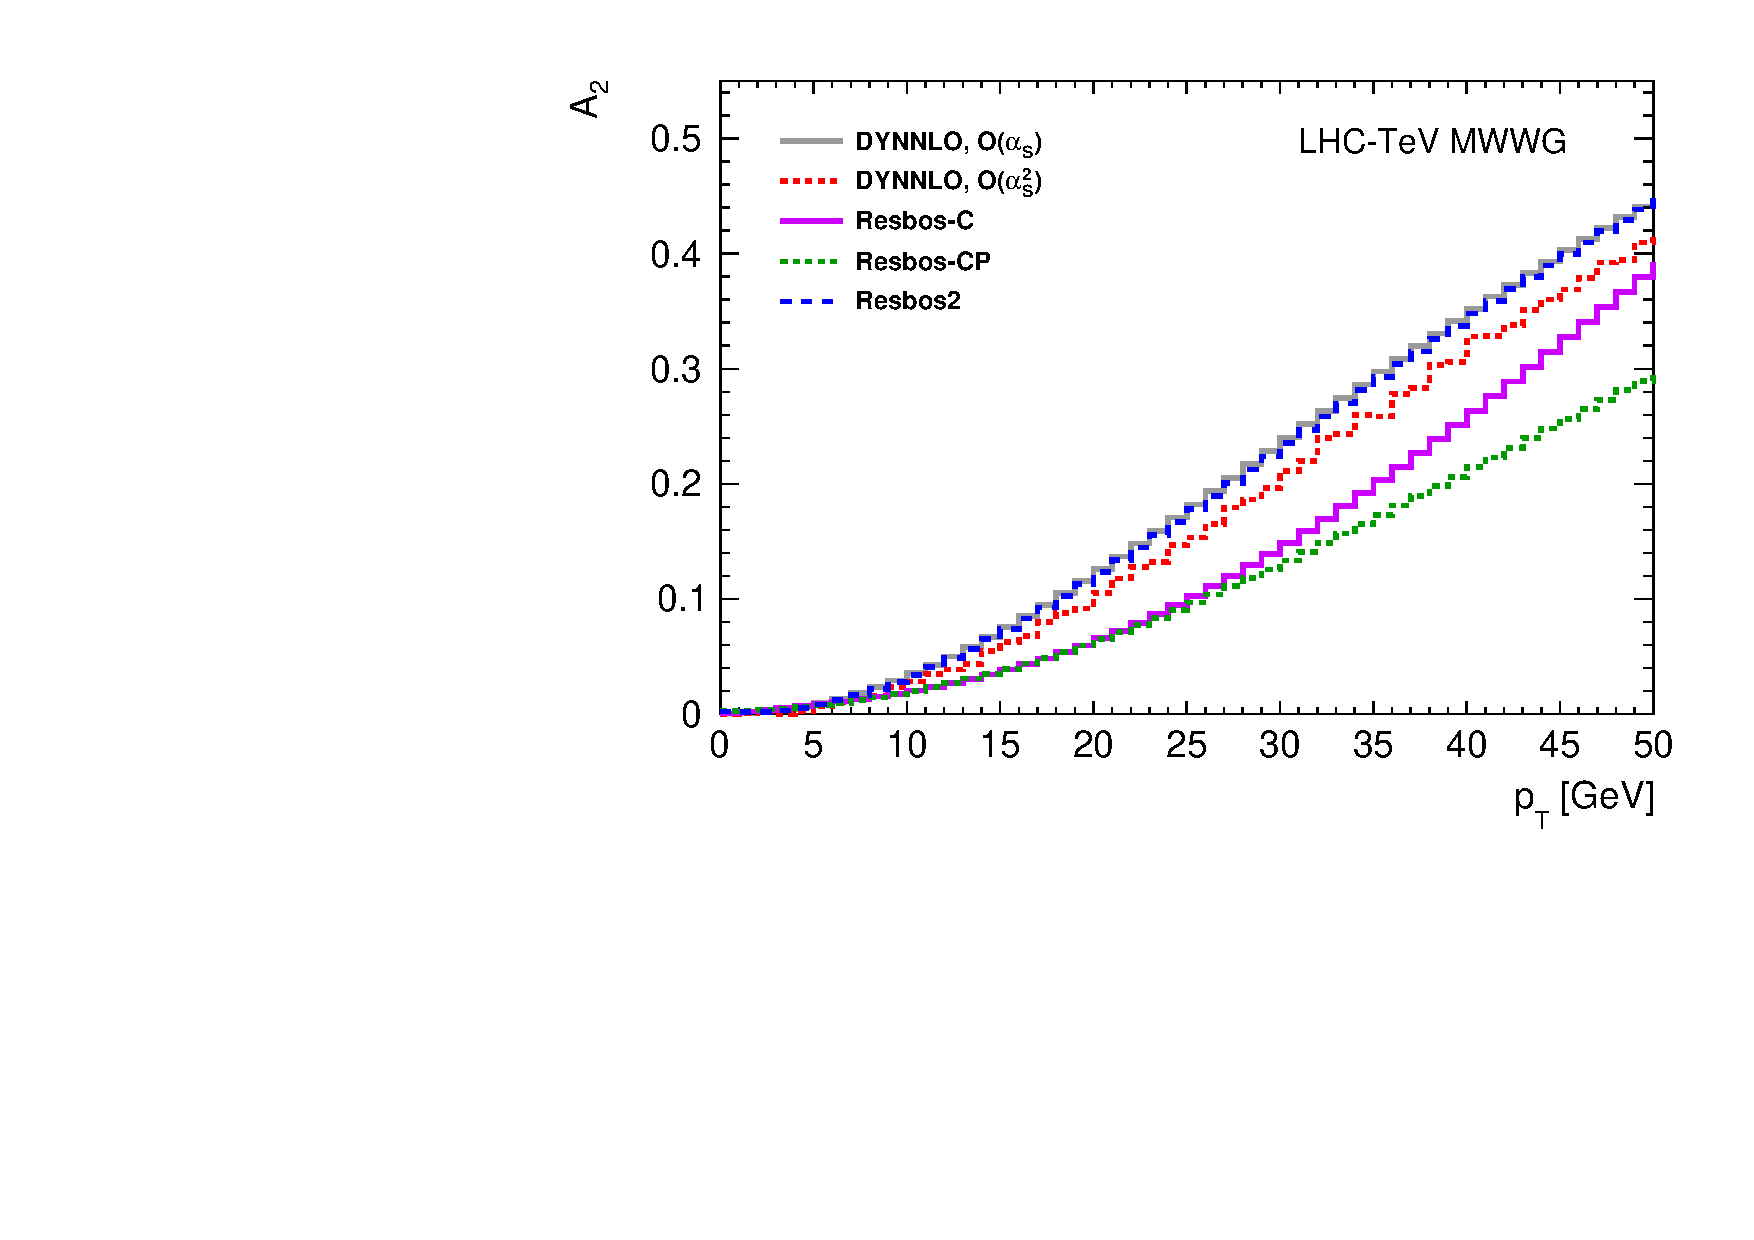
\includegraphics[width=0.88\columnwidth]{a2_pt.pdf}
  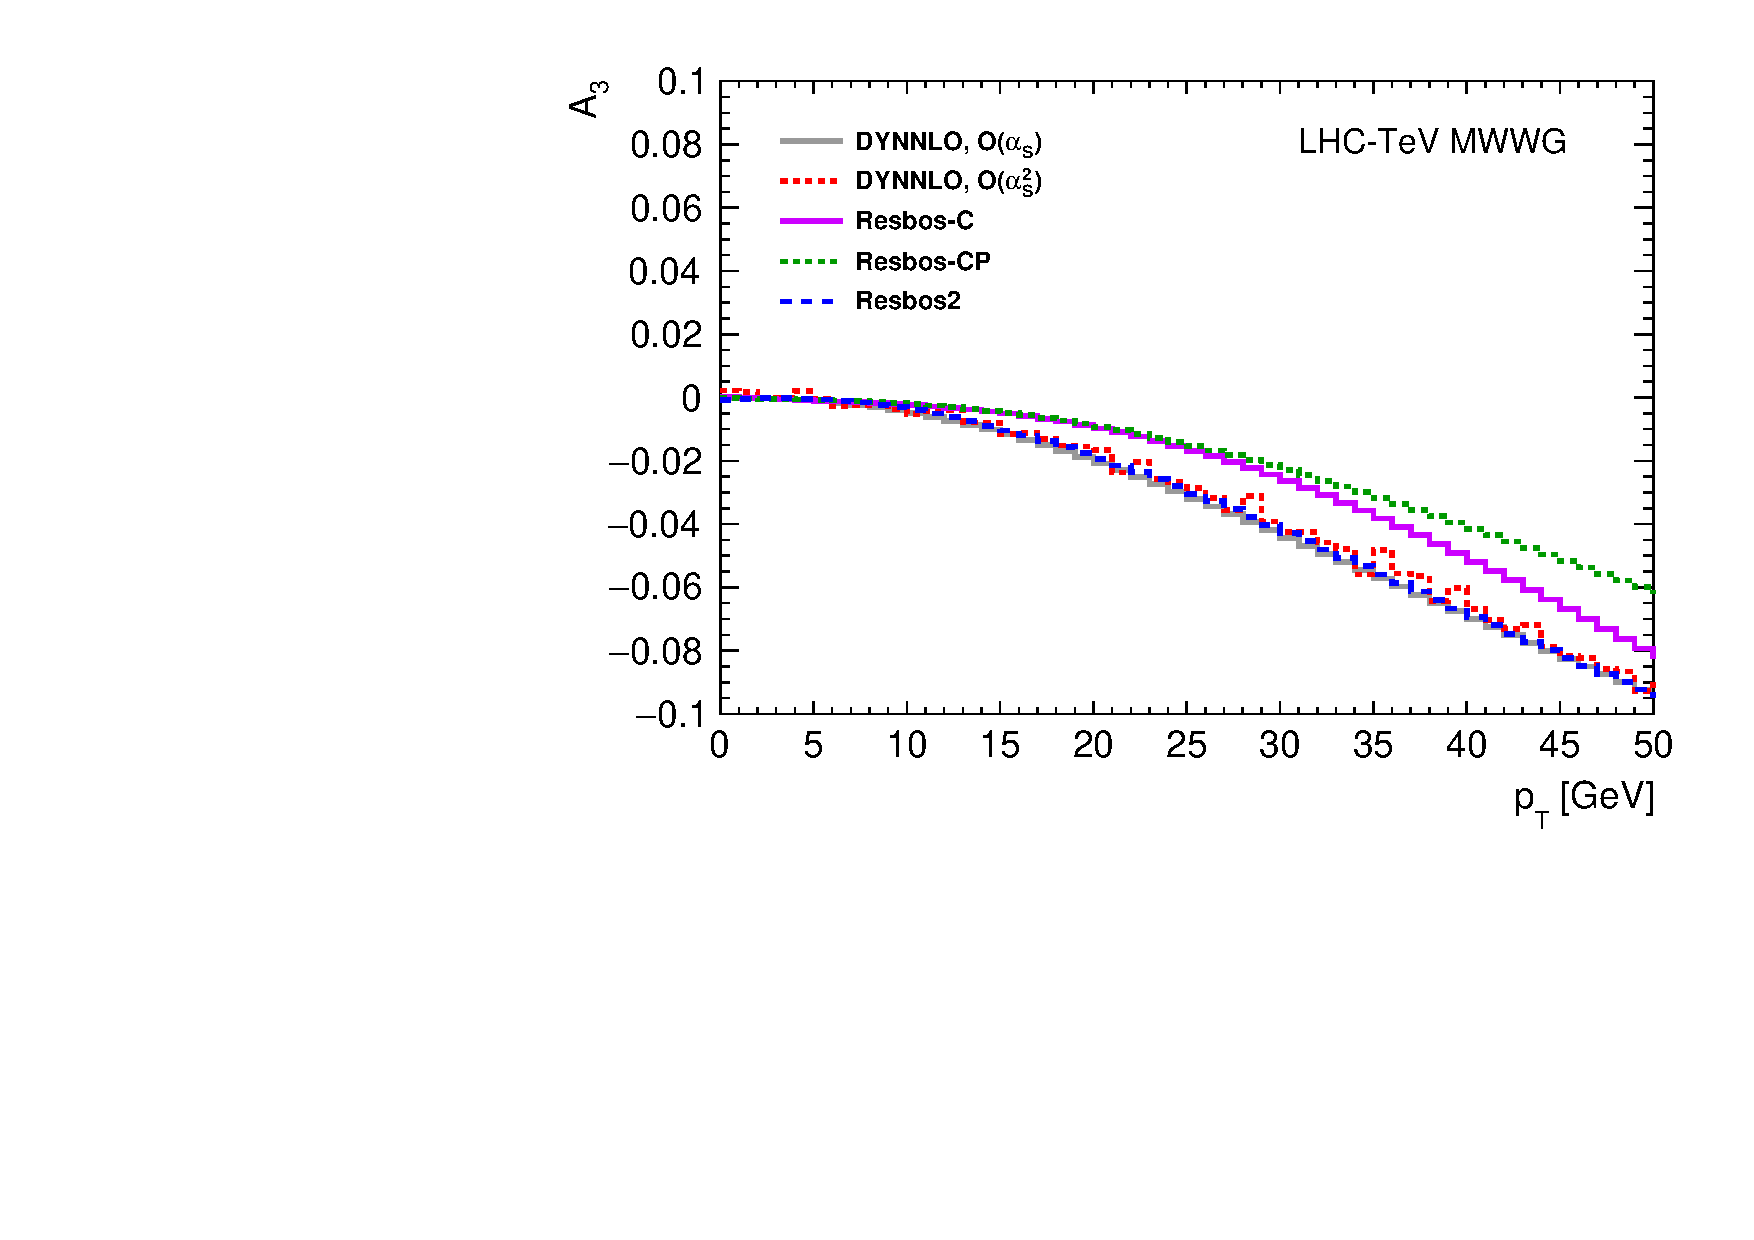
\includegraphics[width=0.88\columnwidth]{a3_pt.pdf}
  \caption{$A_0$ to $A_3$ as a function of \pTW~extracted from 
    \textsc{ResBos-C}, \textsc{ResBos-CP}, \textsc{ResBos2}, \textsc{DYNNLO} at
    ${\cal O}(\alpha_{\scriptsize\textrm{S}})$, and \textsc{DYNNLO} at ${\cal O}(\alpha^2_{\scriptsize\textrm{S}})$
    in $p\bar{p}$ collisions at 1.96 TeV.  The CTEQ6M PDF set is used for all generators except \textsc{ResBos-CP},
    for which CTEQ6.6 is used.  The \textsc{ResBos-C} and \textsc{ResBos2} calculations are at
    ${\cal O}(\alpha_{\mathrm{S}})$ in QCD, and \textsc{ResBos-CP} is at ${\cal O}(\alpha^2_{\scriptsize\textrm{S}})$.
      The difference between DYNNLO at ${\cal O}(\alpha_{\scriptsize\textrm{S}})$ and
      ${\cal O}(\alpha^2_{\scriptsize\textrm{S}})$ has an ${\cal{O}}$(1 MeV) effect on $\delta m_W^{\mathrm{pol}}$.
  }
\label{fig:aiplots}
\end{figure}

\begin{figure}[!htbp]
  \centering
  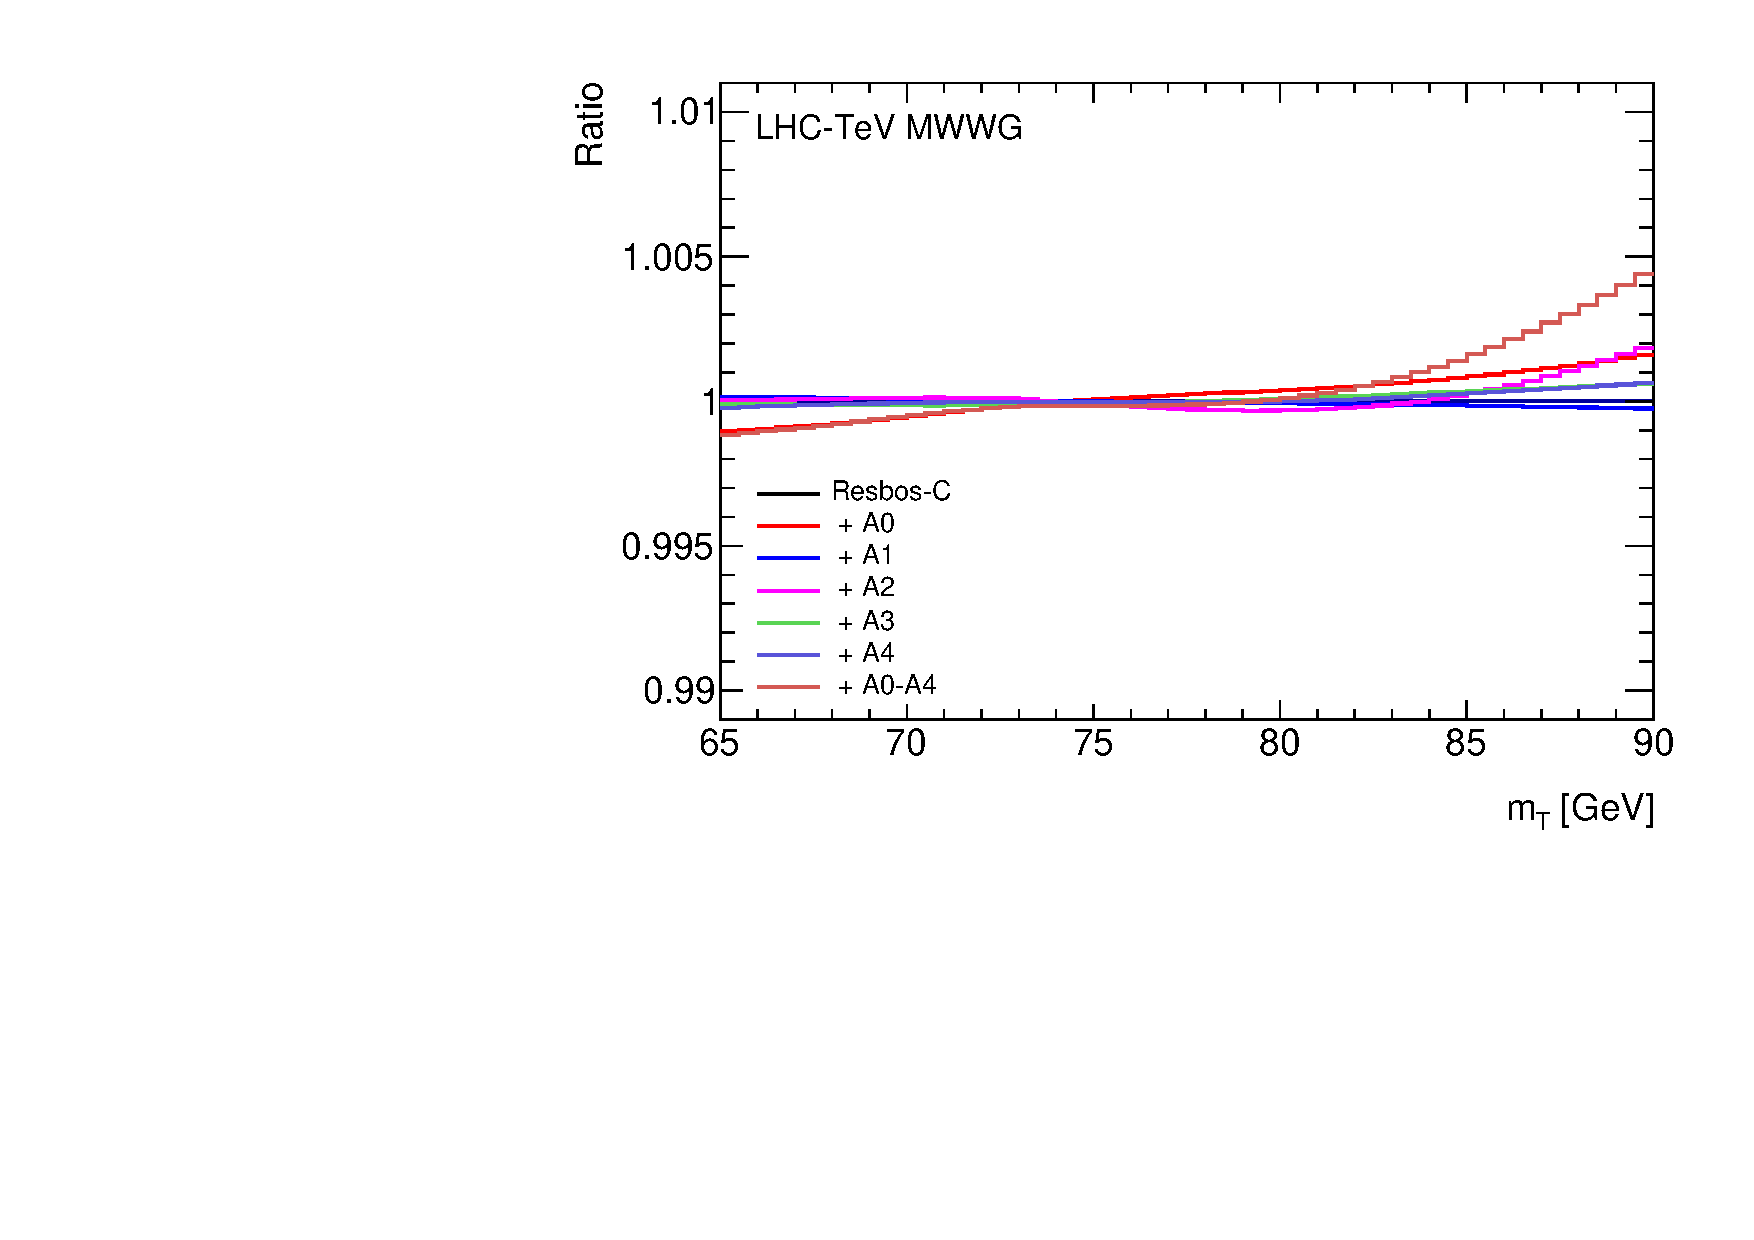
\includegraphics[width=0.9\columnwidth]{mTSmeared_cut7_0_norm_ratio.pdf}
  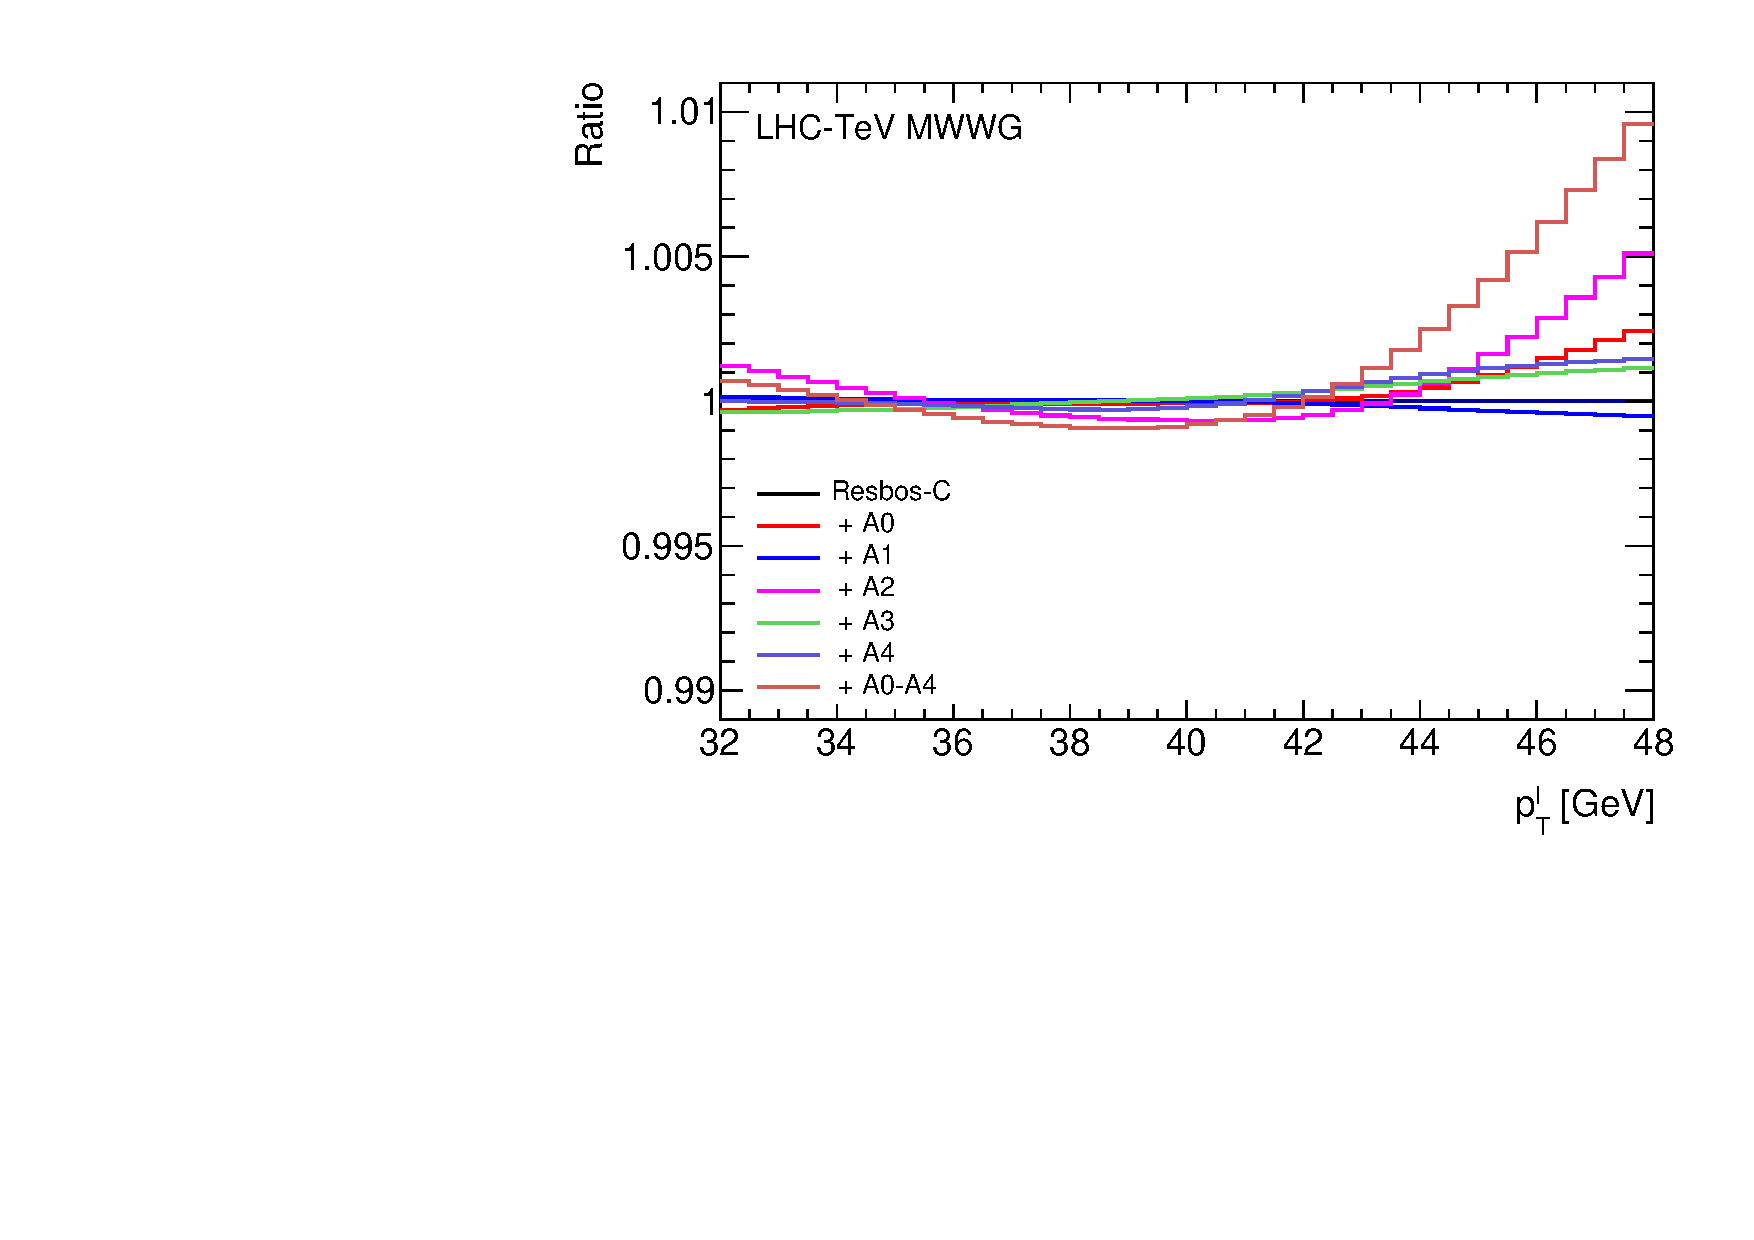
\includegraphics[width=0.9\columnwidth]{muPtsmeared_cut7_0_norm_ratio.pdf}
  \caption{Relative effect of reweighting the $A_0$--$A_4$ coefficients from \textsc{ResBos-C} to 
\textsc{ResBos2} on the CDF \mT~(left) and \pTl~(right) distributions. 
  }
\label{fig:airewCDF}
\end{figure}

\begin{table}[!tbp]
  \centering
  \begin{tabular}{lccc}
    \hline \hline
    Coefficient      &  \mT             & \pTl           & \pTnu   \\
    \hline
    $A_0$            &  $-6.3$          & $-2.6$         & $-9.1$     \\
    $A_1$            &   1.1            &  1.3           &  0.3      \\
    $A_2$            &  $-0.7$          &  0.4           & $-3.2$      \\
    $A_3$            &  $-2.1$          & $-4.1$         &  1.0       \\
    $A_4$            &  $-1.4$          & $-3.3$         & $-1.6$        \\
    $A_0-A_4$        &  $-9.5$          & $-8.4$         & $-12.5$        \\
    \hline
    \textsc{ResBos2} &  $-10.2 \pm 1.1$ & $-7.6 \pm 1.2$ & $-11.8 \pm 1.4$ \\
    \hline 
    Difference       &  $-0.7 \pm 1.1$  &  $0.8 \pm 1.2$ &   $0.7 \pm 1.4$ \\
    \hline \hline
  \end{tabular}
  \caption{Values of $\delta m_W^{\mathrm{pol}}$ in MeV associated with reweighting each $A_i$ coefficient from
    {\textsc{Resbos-C}} to {\textsc{Resbos2}} for the CDF detector, as well as the result of a direct fit
    to {\textsc{ResBos2}}.  The result of the direct fit is consistent with that of the reweighting. }
\label{tab:aireweightcdf}
\end{table}

\begin{table}[!tbp]
  \centering
  \begin{tabular}{lccc}
    \hline \hline
    Coefficient      &  \mT         & \pTl     & \pTnu \\
    \hline
    $A_0$            &  $-9.8$      & $-7.3$   & $-15.6$ \\
    $A_1$            &   1.9        &  2.4     &   1.8 \\
    $A_2$            &   3.0        &  3.3     &  $-2.7$ \\
    $A_3$            &  $-1.6$      & $-2.9$   &   0.4 \\
    $A_4$            &   0.2        & $-2.3$   &   0.5 \\
    $A_0-A_4$        &  $-6.4$      & $-6.9$   & $-15.8$ \\
    \hline
    \textsc{ResBos2} & $-7.8 \pm 1.0$ & $-6.6 \pm 1.1$ & $-16.5 \pm 1.2$ \\
    \hline 
    Difference       & $-1.4 \pm 1.0$ & $0.3 \pm 1.1$  & $-0.7 \pm 1.2$ \\
    \hline \hline
  \end{tabular}
  \caption{Values of $\delta m_W^{\mathrm{pol}}$ in MeV associated with reweighting each $A_i$ coefficient from
    {\textsc{ResBos-CP}} to {\textsc{Resbos2}} for the D0 detector, as well as the result of a direct fit to 
{\textsc{ResBos2}}.  The result of the direct fit is consistent with that of the reweighting. }
\label{tab:aireweightd0}
\end{table}
